\section{Background}

\subsection{CryptDB}\label{CryptDB}
CryptDB is a system that reconciles practicability and confidentiality for applications that use database management systems(DBMSes). 

It encrypts private data in DBMSes with onions of encryption to prevent curious database administrators. 
Applications could still execute queries over encrypted data using a collection of efficient SQL-aware encryption schemes. 
Unlike traditional C/S architecture that web servers issue SQL queries to back-end servers running DBMSes directly as illustrated in figure~\ref{fig:stack1}(a). 
CryptDB puts a proxy server, as illustrated in figure~\ref{fig:stack1}(b), between the web server and DBMS server which intercepts all SQL queries and rewrites them to execute on encrypted data. 
The results are sent back to the proxy server first for decryption, and then plain text will be sent to web server. 
The decryption keys will be kept in proxy servers where we trust so the DBMS server never see sensitive data.


% \subsection{Structure of Cryptdb}

% In the cryptdb system, there are three components: client, server, and proxy. The Client is usually a webserver, and the server has MySQL  or other DBMS installed. In our current environment, we use MySQL5.7 as DBMS and MySQL-Proxy0.8.5 as proxy. The client communicate with the proxy instead of communicating directly with the server. The MySQL server is not trusted while the Proxy is trusted. When the client receive DDL queries, it will stored related encryption metadata to describe the encryption scheme of each table. For both DML and DDL queries, the proxy perform query rewrite to encrypt the query and send encrypted query to MySQL server. The results are sent to the proxy first for decryption, and then plain text will be sent to client. Figure~\ref{fig:stack1} shows the four steps of executing a SQL query in a system using Cryptdb and the two steps of executing SQL queries in a system using normal database system.


\begin{figure}[tb]
\centering
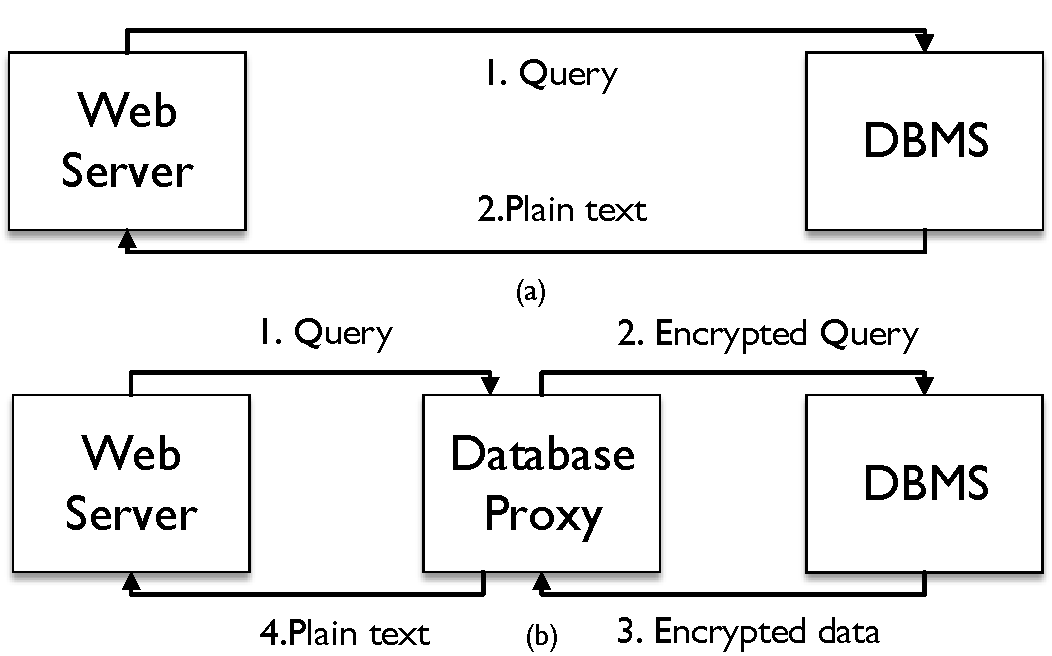
\includegraphics[width=6cm]{images/Cryptdb-structure.pdf}
\caption{(a) shows the normal interaction between the web server and the DBMS, (b) shows the four steps of query execution in a cryptdb system}
\label{fig:stack1}
\end{figure}

% \subsection{metadata layout and structure}

% This section talks about metadata layout and the corresponding encryption scheme. Those scheme will impact how we make choices when we bakcup data. The metadata form a hierarchy from the database level to the encryption layer level. It has a structure of a tree. Figure~\ref{fig:stack2} shows the structure of onionmeta.

CryptDB leverages \emph{onions of encryption} to minimize the information revealed to the untrusted DBMS server. 
\emph{Onions of encryption} dress each value in layers of increasingly stronger encryption. 
Each layer of each onion enables certain kinds of functionality and also leaks certain kinds of information.
The outermost layers usually provide maximum security with no functionality.
The layer of encryption could be adjusted dynamically according to the requested queries. 

To builds the hierarchy of security level, CryptDB uses a number of encryption types:\textit{Random (RND)}, \textit{Deterministic (DET)}, \textit{Order-preserving encryption (OPE)}, \textit{Homomorphic encryption (HOM)}, \textit{Join (JOIN and OPE-JOIN)}, \textit{Word search (SEARCH)}.
RND provides the maximum security which maps two equal values to different ciphertext. DET supports equal comparison. OPE has the property of order preserving. SEARCH allows searching on cipher text. HOM allows addition on ciphertext. We take two data types, \emph{string} and \emph{integer}\footnote{Currently CryptDB only supports these two data types}, for example. As illustrated in figure~\ref{fig:stackx}, the original value is replicated for three times and encrypted using three different onions, the forth column IV is 64bits random integer used for encryption and decryption of the replicated columns. The onion is binded with several encryption layers, and each layer has it's own encryption key. If we want equal comparison, we can use the onion DET. If we need order comparison like order by, we can use the onion OPE. So different onion support different operation on the ciphertext. If the application issues no queries that compare data items in a column, or that sort a column, the column should be encrypted with RND.


% Currently CryptDB only supports two data types: \emph{string} and \emph{integer}. 
% Figure~\ref{fig:stackx} shows how the data columns of the original plain text table are extended. For integer type, one original column is replicated for three times and encrypted using three different onions, the forth column IV is 64bits random integer used for encryption and decryption of the replicated columns. The column of Integer type is also replicated three times. And IV is used for the same purpose. Each of the replicated column is called an onion column. The onion is binded with several encryption layers, and each layer has it's own encryption key. The name of the onion columns indicates the onion's function: Onion  So the queries for the web server against the columns on the original table is transformed into queries against the encrypted onion columns. If we want equal comparison, we can use the onion DET. If we need order comparison like order by, we can use the onion OPE. So different onion support different operation on the ciphertext. 


\begin{figure}[tb]
\centering
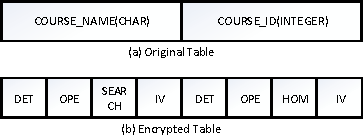
\includegraphics[width=6cm]{images/Extended.pdf}
\caption{(a) is an plain text table with two columns, and (b) is the coresponding encrypted table. Each column is replicated three times, and encrypted using three different onions, Onion means layers of encryption. An additional IV column is stored, which is used together with the decryption key to decrypt the RND layers of the onions}
\label{fig:stackx}
\end{figure}

For security purposes, each onion also have two or more layers. Figure~\ref{fig:stack2}(a) provides illustration of the onions for string, and Figure~\ref{fig:stack2}(b) shows the layout of the onions for integer type. We can find that in each onion, the original plain text is encrypted several times through layers of encryption. For example, onion O-DET-STR has three layers. Suppose that the plaintext is 'p1', and it is first encrypted using AES\_CMC, and we get the ciphertext 'c1'. Then in the second layer DET\_STR, 'c1' is used as input and we still use AES\_CMC for encryption, the result is 'c2'. Finally in the RND\_STR layer, AES\_CBC is used, and we get the final result 'c3'. It should be noted that random IV is used for encryption in the RND layer. So for this O-DET-STR column, two identical values are still the same in the first two layers, However, they are different when they reach the third layer because IV is used together with encryption key for encryption in this layer. Since each row in the table has thier own random IV for each field, the ciphertext for identical plaintext may not be identical. 

Different layers of one onion provide different level of security and also different function. The layer RND is random, so it can not provide any function. The layer DET-STR allow equal comparison, and the layer DET-JOIN-STR allow equal join operation between two tables. It should be noted that the onion DET only support equal comparison operation, and no layer of this onion can support order comparison or other functions. So in summary, each onion support one kind of operation, and each level of the onion reveal different level of that ability.





\begin{figure}[tb]
\centering
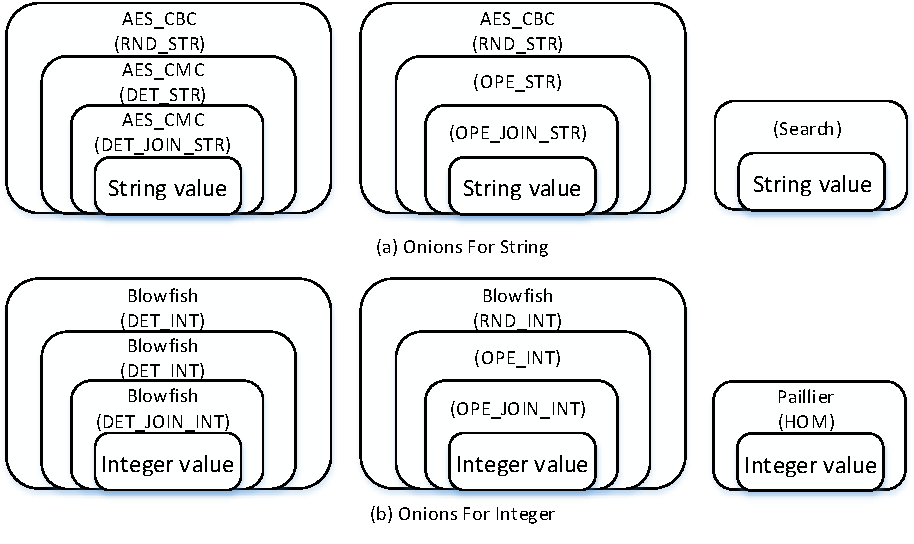
\includegraphics[width=8cm]{images/Onions.pdf}
\caption{(a)describes the three onions for data of String type.(b)describes the three onions for data of Integer type.}
\label{fig:stack2}
\end{figure}


The proxy server in CryptDB stores the metadata and decryption keys. It records the encryption details of the table in the DBMS. For example, we can read and parse the metadata to find how many databases are created. For each database, we can find how many table are in it. For each table, we can find how many fields it has, and for each field, the detailed information of the onions and layers are recorded. Those information will impact how we make choices when we backup data. The metadata form a hierarchy from the database level to the encryption layer level. It has a structure of a tree, and is encoded and stored in a relational table. The amount of metadata is related only to the number tables and the number of fields in those tables, so the storage size is relatively small.

% Figure~\ref{fig:stack2} shows the structure of onionmeta. This is the information we need for logical deduplication. 



% \begin{figure}[tb]
% \centering
% 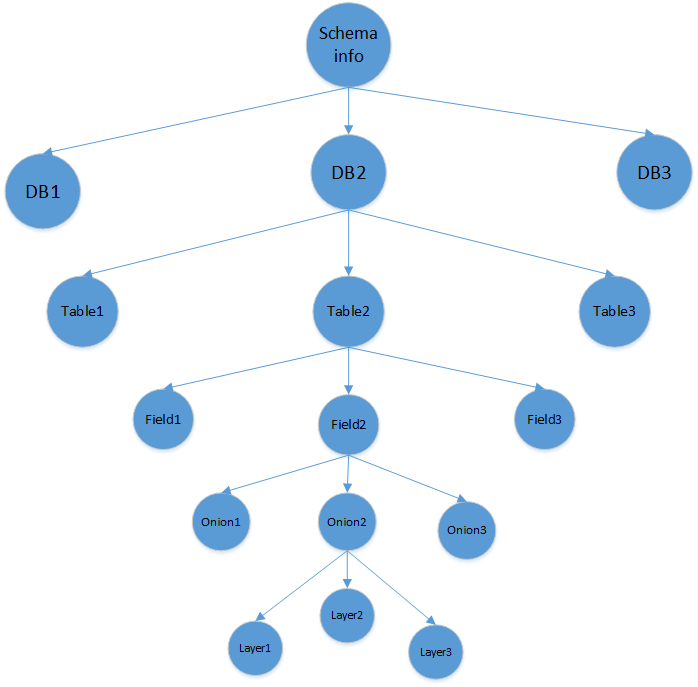
\includegraphics[width=4cm]{images/layers.png}
% \caption{Onionmeta layout}
% \label{fig:stack3}
% \end{figure}


% Every node in the tree is storaed as a record with a unique id in a relational table. The relation among nodes and the content of a node is also stored in the same table. Each onion represents an encryption scheme, which has many layers. This tree structure can be stored in a simple relational table, 

% % CREATE TABLE MetaObject(id bigint(20) unsigned auto\_increment, parent\_id bigint(20),serial\_key varbinary(500),serial\_object varbinary(500));  


% So the metadata of databases, tables, fields, onions, layers are all serialized and stored in the proxy. 

% Since the amount of data is related only to the number tables and the number of fields in those tables, the storage size is small. Also, metadata is needed for decryption and data recovery, so we use physical backup and do not deduplicate the metadata. Metadata is in the form is plaintext, so traditional deduplication techinques can work properly.


